\documentclass{article}
\usepackage{graphicx} % Required for inserting images
\usepackage{quantikz}
\usepackage{physics}
\usepackage{amssymb}
\usepackage[margin = 2cm]{geometry} 
\usepackage{hyperref}
\usepackage{minted}

\usepackage{quantikz}

\begin{document}

\noindent {\Huge \textbf{$\hat Q\ket{B}$asics}}\\
{\large \textbf{Activity 3:} Outer products, operators, and circuits\\

\section*{Resolution of the identity}
\subsection*{In two dimensions}
Suppose that $\ket{i}, \ket{j}$ form an orthonormal basis for $\mathbb C^2$. Show that
$$
\ketbra{i}{i} + \ketbra{j}{j} = I
$$
where $I$ is the identity operator.  \\ \\

\noindent \textit{Note: this identity generalizes to $d$ dimensions. If $\{\ket{n}\}_{n=0}^{d-1}$ is an orthonormal basis for $\mathbb C^d$, then}
$$
\sum_{n=0}^{d-1}\ketbra{n}{n} = I
$$
\subsection*{Solution}
A linear operator is completely defined by its action on any orthonormal basis. $\{\ket{i}, \ket{j}\}$ is orthonormal implies that
\begin{align*}
    \braket{i}{i} &= \braket{j}{j} = 1 \\
    \braket{i}{j} &= 0
\end{align*}
Multiplication of kets is distributive, so we have
$$
(\ketbra{i}{i} + \ketbra{j}{j})\ket{i} = \ket{i}\underbrace{\braket{i}{i}}_{=1} + \ket{j} \underbrace{\braket{j}{i}}_{=0} = I\ket{i}
$$
Similarly, 
$$
(\ketbra{i}{i} + \ketbra{j}{j})\ket{j} = \ket{j}\underbrace{\braket{i}{j}}_{=0} + \ket{j} \underbrace{\braket{j}{j}}_{=1} = I\ket{j}
$$
Since they act the same way on an orthonormal basis, 
$$
(\ketbra{i}{i} + \ketbra{j}{j}) = I
$$
\section*{Unitary operators}
\subsection*{Unitary operators preserve inner products}
We defined a \textit{unitary} operator as a linear operator that conserves total probability, i.e. 
$$
\bra{\psi}U^\dagger U \ket{\psi} = \Vert U\ket{\psi} \Vert^2  = \Vert \ket{\psi} \Vert^2 = 1
$$
Using the fact that this is true for an arbitrary state $\ket{\psi}$, prove that $U^\dagger U = I$, where $I$ is the identity operator.\\ \\
\noindent \textit{Hint: Consider the states $\frac{\ket{0} + \ket{1}}{\sqrt{2}}$ and $\frac{\ket{0} + i\ket{1}}{\sqrt{2}}$.}

\subsection*{Solution}
Let $\ket{\phi} = (\ket{0}+\ket{1})/\sqrt{2}$. We can check that $\Vert \ket{\phi} \Vert^2 = 1$. By the probability-conserving property,
$$
\bra{\phi}U^\dagger U \ket{\phi} = 1
$$
We can also expand this in terms of $\ket{0}, \ket{1}$:
\begin{align}
\bra{\phi}U^\dagger U \ket{\phi} &= \qty(\frac{\bra{0} + \bra{1}}{\sqrt{2}})U^\dagger U \qty(\frac{\ket{0} + \ket{1}}{\sqrt{2}}) \\
&= \frac{\bra{0}U^\dagger U\ket{0} + \bra{1}U^\dagger U\ket{0} + \bra{0}U^\dagger U\ket{1} + \bra{0}U^\dagger U\ket{0}}{2}
\end{align}
By the probability-conserving property, we have $\bra{0}U^\dagger U \ket{0} = 1$ and $\bra{1}U^\dagger U \ket{1} = 1$. As a general property of the adjoint operation, we also have
$$
\bra{1}U^\dagger U\ket{0} = (\bra{0}U^\dagger U\ket{1})^\ast
$$
Where ${}^\ast$ denotes the complex conjugate. This gives
\begin{align}
\frac{\bra{0}U^\dagger U\ket{0} + \bra{1}U^\dagger U\ket{0} + \bra{0}U^\dagger U\ket{1} + \bra{1}U^\dagger U\ket{1}}{2} &= \frac{2 + 2\Re(\bra{0}U^\dagger U \ket{1})}{2} = 1 
\end{align}
This top equation implies that $\Re(\bra{0}U^\dagger U \ket{1}) = 0$. We can repeat the same process with $\ket{\psi} = (\ket{0}+i\ket{1})/\sqrt{2}$. We get
\begin{align}
\bra{\psi}U^\dagger U \ket{\psi} &= \qty(\frac{\bra{0} -i\bra{1}}{\sqrt{2}})U^\dagger U \qty(\frac{\ket{0} + i\ket{1}}{\sqrt{2}}) \\
&= \frac{\bra{0}U^\dagger U\ket{0} - i\bra{1}U^\dagger U\ket{0} + i\bra{0}U^\dagger U\ket{1} + \bra{1}U^\dagger U\ket{1}}{2} \\
&= \frac{2 + 2i\Im(\bra{0}U^\dagger U\ket{1})}{2} = 1
\end{align}
The last equation implies that $\Im(\bra{0}U^\dagger U \ket{1}) = 0$. Together, we have $\bra{0}U^\dagger U \ket{1} = 0$ and $\bra{1}U^\dagger U \ket{0} = (\bra{0}U^\dagger U \ket{1})^\ast = 0$. This implies that $U^\dagger U\ket{0} = \alpha \ket{0}$ and $U^\dagger U \ket{1} = \beta\ket{1}$, where $\alpha$ and $\beta$ are constants. Since $\bra{0}U^\dagger U \ket{0} = \alpha = 1$ and $\bra{1}U^\dagger U \ket{1} = \beta = 1$, we have $U^\dagger U\ket{0} = \ket{0}$ and $U^\dagger U \ket{1} = \ket{1}$. This shows that $U^\dagger U = I$.

\subsection*{Pauli-Euler identity}
Consider again the Pauli-$X$ operator, defined by $X \ket{0} = \ket{1}$ and $X \ket{1} = \ket{0}$. Recall from last time that the $X-$basis is defined as
\begin{align}
\ket{+} &= \frac{\ket 0 + \ket 1}{\sqrt{2}} &
\ket{-} &= \frac{\ket 0 - \ket 1}{\sqrt{2}}
\end{align}
Since $X\ket{+} = \ket{+}$ and $X \ket{-} = -\ket{-}$, we can consistently define $e^{i\theta X}\ket{+} = e^{i\theta}\ket{+}$ and $e^{i\theta X}\ket{-} = e^{-i\theta}\ket{-}$. Using this, show that
$$
e^{i\theta X} = I\cos(\theta) + i X\sin(\theta)
$$
where $I$ is the identity operator.\\ \\
\noindent \textit{Note: This holds for any operator that is self-inverse because these operators have eigenvalues $\pm 1$, including $Y$, $Z$, and $n_xX + n_yY + n_zZ$ where $\Vert (n_x, n_y, n_z) \Vert = 1$.}

\subsection*{Solution}
We can specify a linear operator by its action on an orthonormal basis, and $\ket{+}, \ket{-}$ forms such a basis. Using the Euler formula, we have
$$
(I\cos(\theta) + iX\sin(\theta))\ket{+} = (\cos(\theta) + i\sin(\theta))\ket{+} = e^{i\theta}\ket{+}
$$
and
$$
(I\cos(\theta) + iX\sin(\theta))\ket{-} = (\cos(\theta) - i\sin(\theta))\ket{-} = e^{-i\theta}\ket{-}
$$
This shows that $e^{i\theta X} = I\cos(\theta) + iX\sin(\theta)$.

\section*{The trace}
The \textit{trace} is a useful operation in quantum mechanics. The trace of an operator $\hat{ O}$ is defined
$$
\Tr{\mathcal O} = \bra{0}\mathcal O \ket{0} + \bra{1} \mathcal O \ket{1}
$$
If we write $\mathcal O$ using outer products,
$$
\mathcal O = \mathcal O_{00}\ketbra{0}{0} + \mathcal O_{10}\ketbra{1}{0} + \mathcal O_{01}\ketbra{0}{1} + \mathcal O_{11}\ketbra{1}{1}
$$
we can see that $\Tr{\mathcal O} = \mathcal O_{00} + \mathcal O_{11}$, which is just the standard definition of the trace as the sum of diagonal elements. In $d$ dimensions, if $\{\ket{n}\}_{n=0}^d$ is an orthonormal basis for $\mathbb C^d$, then the trace can be similarly defined as
$$
\Tr{\mathcal O} = \sum_{n}\bra{n}\mathcal O \ket{n}
$$

\subsection*{Cyclic property of the trace}
Let $A$ and $B$ both be operators on a $d-$dimensional complex vector space. Using the resolution of the identity, show that
$$
\Tr{AB} = \Tr{BA}
$$

\subsection*{Solution}
Note that $\bra{n}A\ket{m}$ is just a scalar, so it commutes with everything. Then using the defintion of the trace and resolution of the identity, we have
\begin{align}
\Tr{AB} &= \sum_{n=0}^{d-1}\bra{n}AB\ket{n} \\
&= \sum_{n=0}^{d-1}\bra{n}A\sum_{m=0}^{d-1}\ketbra{m}{m}B\ket{n} \\
&= \sum_{m=0}^{d-1}\sum_{n=0}^{d-1}\bra{n}A\ketbra{m}{m}B\ket{n} \\
&= \sum_{m=0}^{d-1}\sum_{n=0}^{d-1}\bra{m}B\ketbra{n}{n}A\ket{n} \\
&= \sum_{m=0}^{d-1}\bra{m}B\sum_{n=0}^{d-1}\ketbra{n}{n}A\ket{m} \\
&= \sum_{m=0}^{d-1}\bra{m}BA\ket{m} = \Tr{BA}
\end{align}

\subsection*{Unitary invariance of trace}
If $\{\ket{i}\}_{i = 0}^{d-1}$ and $\{ \ket{j}\}_{j=0}^{d-1}$ are two different orthonormal bases, then the operator $U$ such that $U\ket{i} = \ket{j}$ is unitary. Use this to show that the trace is invariant with respect to the choice of basis:
$$
\Tr\{\mathcal O\} = \sum_{i}\bra{i}\mathcal O \ket{i} = \sum_{j}\bra{j}\mathcal O \ket{j}
$$
\textit{Note: This is a slight abuse of notation because the labels $i$ and $j$ are both denoting indices and distinguishing between the two bases.} 

\subsection*{Solution}
Let $\Tr{O} = \sum_{i}\bra{i}\mathcal O\ket{i}$, and take $\ket{j} = U\ket{i}$. Since $U$ is unitary, we have $U^\dagger U = UU^\dagger = I$. By the cyclic property of the trace,
$$
\sum_{j}\bra{j}\mathcal O \ket{j} = \sum_{i}\bra{i}U^\dagger\mathcal O U\ket{i} = \Tr{U^\dagger \mathcal O U} = \Tr{\mathcal O U U^\dagger} = \Tr{\mathcal O}
$$

\section*{Hello Quantum World}
\subsection*{The Hadamard gate}
The Hadamard gate is used to create superpositions, and it is defined as
\begin{align}
    H \ket{0} &= \ket{+} \\
    H\ket{1} &= \ket{-}
\end{align}
Make the following circuit in Qiskit:
\begin{quantikz}
  \ket{0} & \gate{H} & \meter{} \qw
\end{quantikz}.
Recall that the definition of the $Z$ operator is $Z\ket{0} = \ket{0}$ and $Z \ket{1} = -\ket{1}$, and the expectation value is defined as $\langle Z \rangle = \bra{\psi}Z\ket{\psi}$. Can you predict the expectation value $\langle Z \rangle?$ Confirm your prediction by simulating in Qiskit.

\subsection*{Solution}
For a generic state $\psi = \alpha \ket{0} + \beta\ket{1}$, the expectation value of $Z$ is
\begin{align*}
\langle Z \rangle \equiv \bra{\psi}Z\ket{\psi} &= \qty(\alpha^\ast \bra{0} + \beta^\ast \bra{1})Z\qty(\alpha \ket{0} + \beta \ket{1}) \\
&= |\alpha|^2\overbrace{\bra 0 Z \ket 0}^{=1} + \alpha^\ast \beta \overbrace{\bra{0}Z \ket{1}}^{=0} + \alpha \beta^\ast \overbrace{\bra{1} Z \ket{0}}^{=0} + |\beta|^2 \overbrace{\bra{1}Z\ket{1}}^{=-1}\\
&= |\alpha|^2 - |\beta|^2
\end{align*}
By applying a Hadamard gate to the $\ket{0}$ state, we are left in the state $\ket{+}$, which has $\alpha = \beta = \frac{1}{\sqrt{2}}$. The expectation value of $Z$ is then
$$
|\alpha|^2 - |\beta|^2 = \frac{1}{2} - \frac{1}{2} = 0
$$
We also recognize that $|\alpha|^2$ is the probability given by the Born rule of measuring $\ket{\psi}$ in the state $\ket{0}$ and $|\beta|^2$ is the probability of measuring $\ket{\psi}$ in the state $\ket{1}$. In order to compute $\langle Z \rangle$ experimentally, we can run the experiment many times and average the number of 0's and 1's to estimate $|\alpha|^2$ and $|\beta|^2$. The code in Qiskit is the following:
\begin{minted}{python}
from qiskit import QuantumCircuit, execute
from qiskit.providers.aer import AerSimulator
sim = AerSimulator()
qc = QuantumCircuit(1,1)
qc.h(0)
qc.measure(0,0)
shots = 10000
counts = execute(qc, sim, shots = shots).result().get_counts()
expec_Z = (counts.get("0",0)-counts.get("1",0))/shots
\end{minted}

\subsection*{Rotation gates}
Create the following circuit in Qiskit: \begin{quantikz}
  \ket{0} & \gate{R_x(\theta)} & \meter{} \qw
\end{quantikz},
with the definition
$$
R_x(\theta) \equiv e^{-iX \theta/2}
$$
What will be the expectation value of $Z$ as a function of $\theta$? Make a prediction and confirm it by measuring $\langle Z \rangle$ for values of $\theta$ between $0$ and $2\pi$.

\subsection*{Solution}
We have the Pauli-Euler identity, which gives
$$
e^{-iX\theta/2}\ket{0} = \cos(\theta/2)\ket{0} - i\sin(\theta/2)\ket{1}
$$
Using the formula $\langle Z \rangle = |\alpha|^2 - |\beta|^2$, we get
$$
\langle Z \rangle = \cos^2(\theta/2) - \sin^2(\theta/2) = \cos(\theta)
$$
The code we can use to test this in Qiskit is the following:
\begin{minted}{python}
import numpy as np
def get_expec(theta):
    qc = QuantumCircuit(1,1)
    qc.rx(theta, 0)
    qc.measure(0,0)
    shots = 1000
    counts = execute(qc, sim, shots = shots).result().get_counts()
    return (counts.get("0",0)-counts.get("1",0))/shots
thetalist = np.linspace(0, 2*np.pi, 50)
expects = list(map(get_expec, thetalist))
\end{minted}
\begin{figure}[hbt!]
\centering
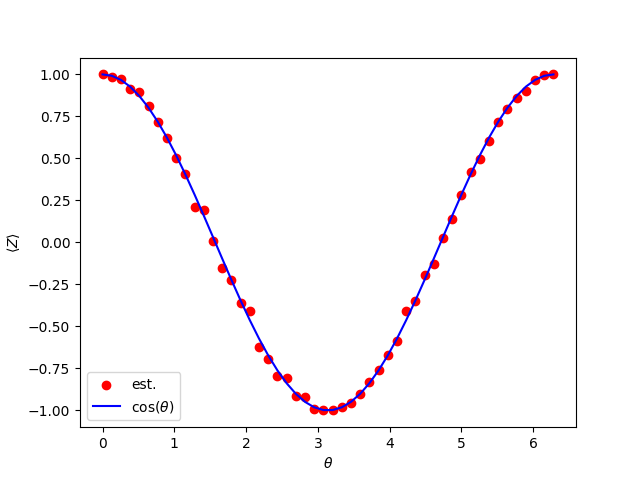
\includegraphics[width = .6\textwidth]{Rabi.png}
\end{figure}
\subsection*{The Bell Basis}
We define the Bell basis as
\begin{align*}
\ket{\Phi_1} &= \frac{\ket{00} + \ket{11}}{\sqrt{2}} & \ket{\Phi_2} &= \frac{\ket{00} - \ket{11}}{\sqrt{2}} \\
\ket{\Phi_3} &= \frac{\ket{01} + \ket{10}}{\sqrt{2}} & \ket{\Phi_4} &= \frac{\ket{01} - \ket{10}}{\sqrt{2}}
\end{align*}

Come up with a circuit to prepare $\ket{\Phi_1}$. Using the definitions
\begin{align*}
X &= \ketbra{1}{0} + \ketbra{0}{1} & Y &= i\ketbra{1}{0} -i\ketbra{0}{1} & Z &= \ketbra{0}{0} - \ketbra{1}{1}
\end{align*}
\begin{itemize}
    \item[(a)] Show that $X_1I_2\ket{\Phi_1} = \ket{\Phi_3}$, $Y_1I_2\ket{\Phi_1} = -i\ket{\Phi_4}$, and $Z_1I_2\ket{\Phi_1} = \ket{\Phi_2}$.
    \item[(b)] Create a circuit that maps $\ket{00}$ to $\ket{\Phi_1}$. Now invert this circuit. What does the inverse do to $\ket{\Phi_2}, \ket{\Phi_3}$, and $\ket{\Phi_4}$?
    \item[(c)] Confirm this prediction in Qiskit.
\end{itemize}
Property (a) reflects a symmetry of $\ket{\Phi_1}$ which makes it a useful resource for superdense coding and quantum teleportation, due to the fact that local (single-qubit) operators are shown to produce nonlocal (multi-qubit) changes to the state.

\subsection*{Part a}
Using the definitions of $X$, $Y$, and $Z$, 
\begin{align*}
    X_1I_2 \ket{\Phi_1} &= \frac{X_1I_2 \ket{00}+X_1I_2 \ket{11}}{\sqrt{2}} \\
    &= \frac{\ket{10}+\ket{01}}{\sqrt{2}} = \ket{\Phi_3}
\end{align*}
\begin{align*}
    Y_1I_2 \ket{\Phi_1} &= \frac{Y_1I_2 \ket{00}+Y_1I_2 \ket{11}}{\sqrt{2}} \\
    &= \frac{i\ket{10}-i\ket{01}}{\sqrt{2}} = -i\ket{\Phi_4}
\end{align*}
\begin{align*}
    Z_1I_2 \ket{\Phi_1} &= \frac{Z_1I_2 \ket{00}+Z_1I_2 \ket{11}}{\sqrt{2}} \\
    &= \frac{\ket{00}-\ket{11}}{\sqrt{2}} = \ket{\Phi_2}
\end{align*}

\subsection*{Part b}
The circuit we want performs the following operation:
$$
\ket{00} \mapsto \frac{1}{\sqrt{2}}(\ket{0} + \ket{1})\ket{0} = \frac{1}{\sqrt{2}}(\ket{00} + \ket{10}) \mapsto \frac{1}{\sqrt{2}}(\ket{00} + \ket{11}) 
$$
The first operation is a Hadamard gate on the first qubit, and the second operation is a CNOT gate controlled on the first qubit and targeting the second qubit. As a circuit,
\begin{center}
\begin{quantikz}[row sep={5mm,between origins}]
  \ket{0} &\gate{H} & \ctrl{1} & \qw \\
  \ket{0} &\qw & \targ{}  & \qw \\
\end{quantikz}
\end{center}
Since $H^{-1} = H$ and $CNOT^{-1} = CNOT$, inverting the circuit is as simple as switching the order of the gates:
\begin{center}
\begin{quantikz}[row sep={5mm,between origins}]
  \qw & \ctrl{1} & \gate{H} & \qw \\
   \qw & \targ{}  & \qw &\qw \\
\end{quantikz}
\end{center}
We can then work out the action of this inverse on the three remaining bell states:
\begin{align*}
    CNOT\ket{\Phi_2} &= \frac{\ket{00} - \ket{10}}{\sqrt{2}} = \qty(\frac{\ket{0}-\ket{1}}{\sqrt{2}})\ket{0} = \ket{-}\ket{0}\\
    H_1I_2\ket{-}\ket{0} = \ket{10}
\end{align*}
\begin{align*}
    CNOT\ket{\Phi_3} &= \frac{\ket{01} + \ket{11}}{\sqrt{2}} = \qty(\frac{\ket{0}+\ket{1}}{\sqrt{2}})\ket{1} = \ket{+}\ket{1}\\
    H_1I_2\ket{+}\ket{1} = \ket{01}
\end{align*}
\begin{align*}
    CNOT\ket{\Phi_4} &= \frac{\ket{01} - \ket{11}}{\sqrt{2}} = \qty(\frac{\ket{0}-\ket{1}}{\sqrt{2}})\ket{1} = \ket{-}\ket{1}\\
    H_1I_2\ket{-}\ket{1} = \ket{11}
\end{align*}
So the inverse maps $\ket{\Phi_2} \mapsto \ket{10}$, $\ket{\Phi_3} \mapsto \ket{01}$, and $\ket{\Phi_4} \mapsto \ket{11}$. In this way, a two-bit message can be encoded by applying only an operation to the first qubit. This is a quantum algorithm known as `superdense coding.'

\subsection*{Part c}
Note: Qiskit follows ``little endian" order, so the qubits are ordered $\ket{q_1q_0}$ instead of $\ket{q_0q_1}$ as above.
\begin{minted}{python}
qc = QuantumCircuit(2)
#prepare |Phi_1>
qc.h(0)
qc.cx(0,1)
#invert
qc.cx(0,1)
qc.h(0)
qc.measure_all()
print(execute(qc, sim).result().get_counts())
#"{'00': 1024}"
\end{minted}
\begin{minted}{python}
qc = QuantumCircuit(2)
#prepare |Phi_2>
qc.h(0)
qc.cx(0,1)
qc.z(0)
#invert
qc.cx(0,1)
qc.h(0)
qc.measure_all()
print(execute(qc, sim).result().get_counts())
#"{'01': 1024}"
\end{minted}
\begin{minted}{python}
qc = QuantumCircuit(2)
#prepare |Phi_3>
qc.h(0)
qc.cx(0,1)
qc.x(0)
#invert
qc.cx(0,1)
qc.h(0)
qc.measure_all()
print(execute(qc, sim).result().get_counts())
#"{'10': 1024}"
\end{minted}
\begin{minted}{python}
qc = QuantumCircuit(2)
#prepare |Phi_4>
qc.h(0)
qc.cx(0,1)
qc.y(0)
#invert
qc.cx(0,1)
qc.h(0)
qc.measure_all()
print(execute(qc, sim).result().get_counts())
#"{'11': 1024}"
\end{minted}
\end{document}
- unitary U|a> = |b> => U is unitary
- expectation of Pauli operators is projection on 3-space
\begin{quantikz}
  \lstick{\ket{0}} & \gate{R_x(\theta)} & \meter{} \qw
\end{quantikz}

\begin{quantikz}
  \lstick{\ket{0}} & \gate{R_x(\theta)} & \meter{} \qw
\end{quantikz}
